\chapter{视觉定位与三维体积测试与分析}
\label{cha:chap5}
\section{引言}
\label{sec:5.1}
做实验做实验做实验
\section{视觉定位系统测试}
\label{sec:5.2}
\subsection{视觉定位系统实验步骤设计}
\label{sec:5.2.1}
在第二章,本文提出了一种结合二维码的SLAM视觉系统,利用该系统可以估计出带有真实尺度的相机位姿,以及能够得到真实世界坐标系下的
相机位置。本次实验主要利用上述方法在复杂封闭,且无GPS信号的环境下,结合二维码视觉标签进行无人机定位,通过获得到的位置信息信
息进行下一步的飞行控制。本次实验的准备过程主要分为三个步骤,布置场景,生成地图,无人机自主循迹。

首先是场景布置,选择在空旷场地中,布置二维码视觉标签,保证每个二维码的尺度大小完全一致,且二维码之间尽可能等间距布置,场景中的
二维码ID完全独立不同,设计图和实际布置图分别如图~\ref{fig:scene_imagine}和图~\ref{fig:scene_reality}所示。在本次实验中,所原选择的二维码实际大小为0.73m,相邻二维码之间的距
离为4m,整个实验区域面积为400m2(20m*20m)。

\begin{figure}[H] % use float package if you want it here
  \centering
  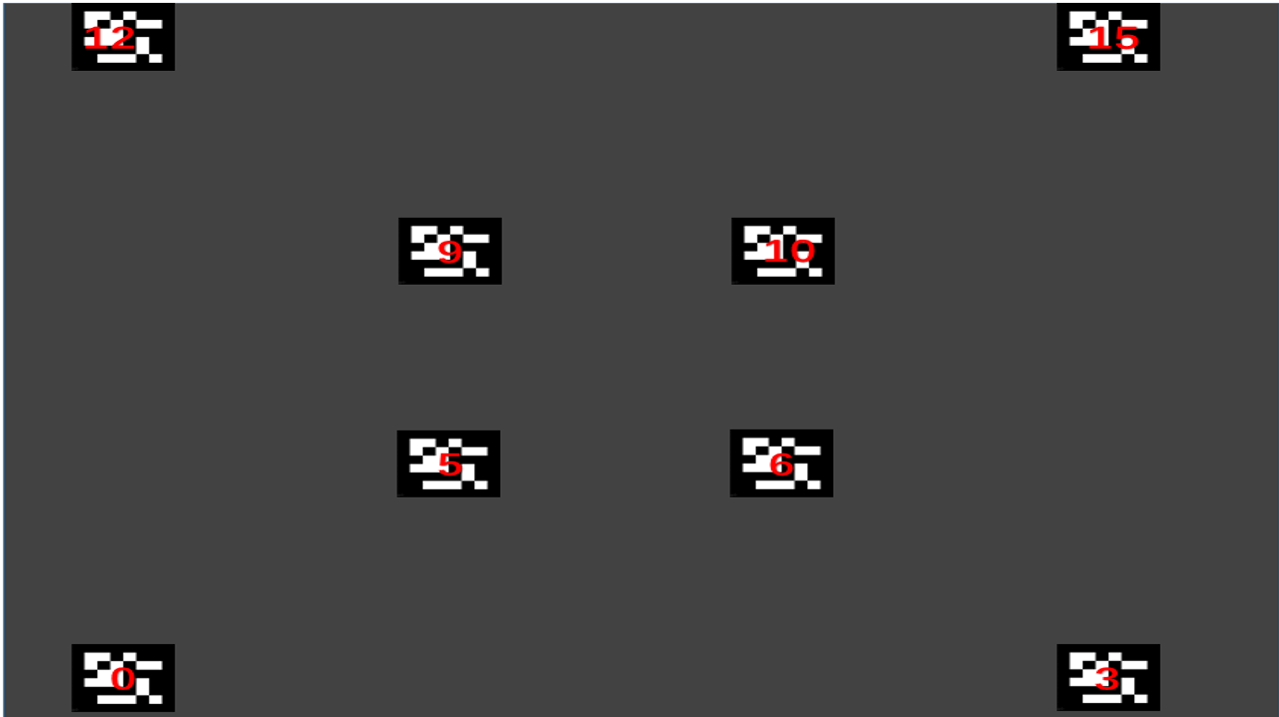
\includegraphics[height=8cm]{scene_imagine.png}
  \caption{实验场景设计示意图}
  \label{fig:scene_imagine}
\end{figure}
\begin{figure}[H] % use float package if you want it here
  \centering
  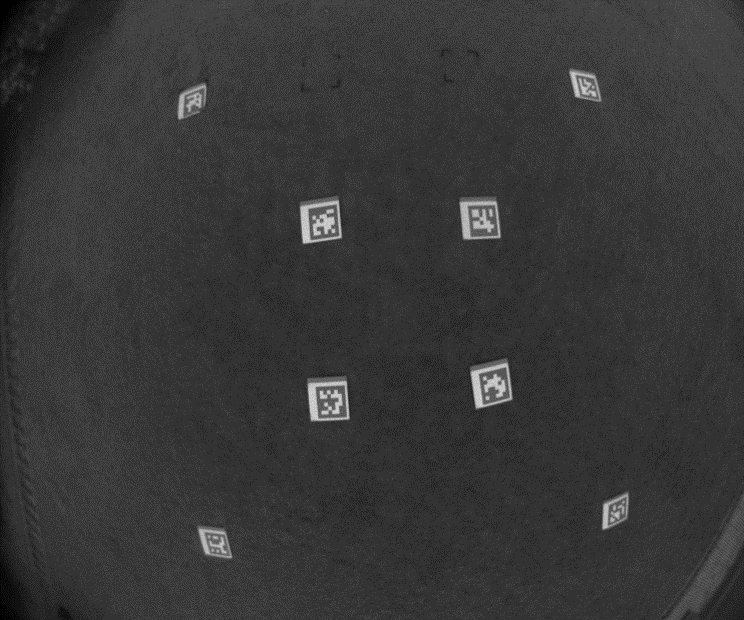
\includegraphics[height=8cm]{scene_reality.png}
  \caption{实验场景真实布置图}
  \label{fig:scene_reality}
\end{figure}

在布置好场景后,需要根据实际场景生成地图信息。当无人机首次在无先验地图的环境下飞行时,需要人工手动控制,完成无人机的飞行和地图
生成工作,在无人机的手动飞行过程中,其飞行区域需要尽可能覆盖所有场景以确保生产完整的地图,根据实际场景生成的地图如图~\ref{fig:map_generator}
所示,其中正方形框代表二维码,蓝色相机表示代表视觉定位产生的关键帧,点代表地图中的特征点。

\begin{figure}[H] % use float package if you want it here
  \centering
  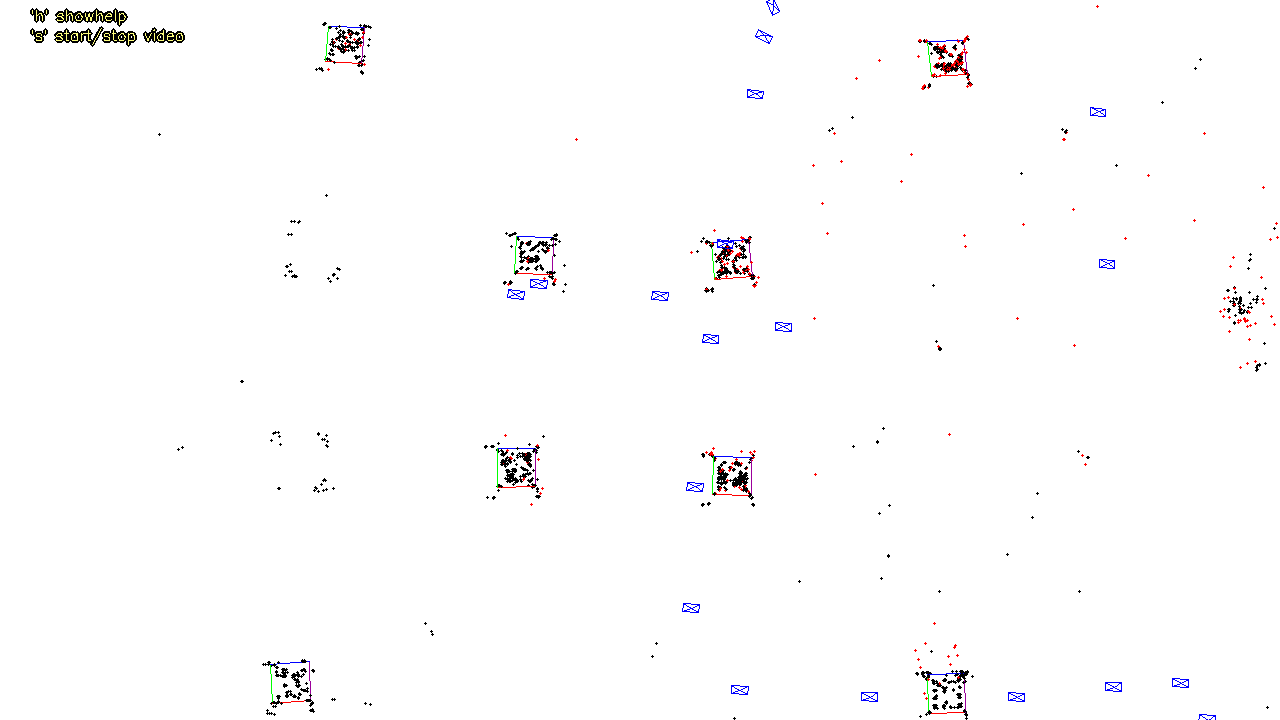
\includegraphics[height=8cm]{map_generator.png}
  \caption{视觉算法生成地图}
  \label{fig:map_generator}
\end{figure}

当获取到完整的地图信息地图后,可以让无人机按照认为规定的轨迹进行自动循迹飞行,首先设计如下图~\ref{fig:flight_route}所示的轨
迹图,其中起始点为ID=0的二维码处,红色箭头代表无人机的飞行轨迹,对于无人机的飞控过程,按照设定循迹点的方案来实现,即在整个轨迹
中给定多个循迹点坐标,使得无人机按照设定的坐标顺序进行飞行。
\begin{figure}[H] % use float package if you want it here
  \centering
  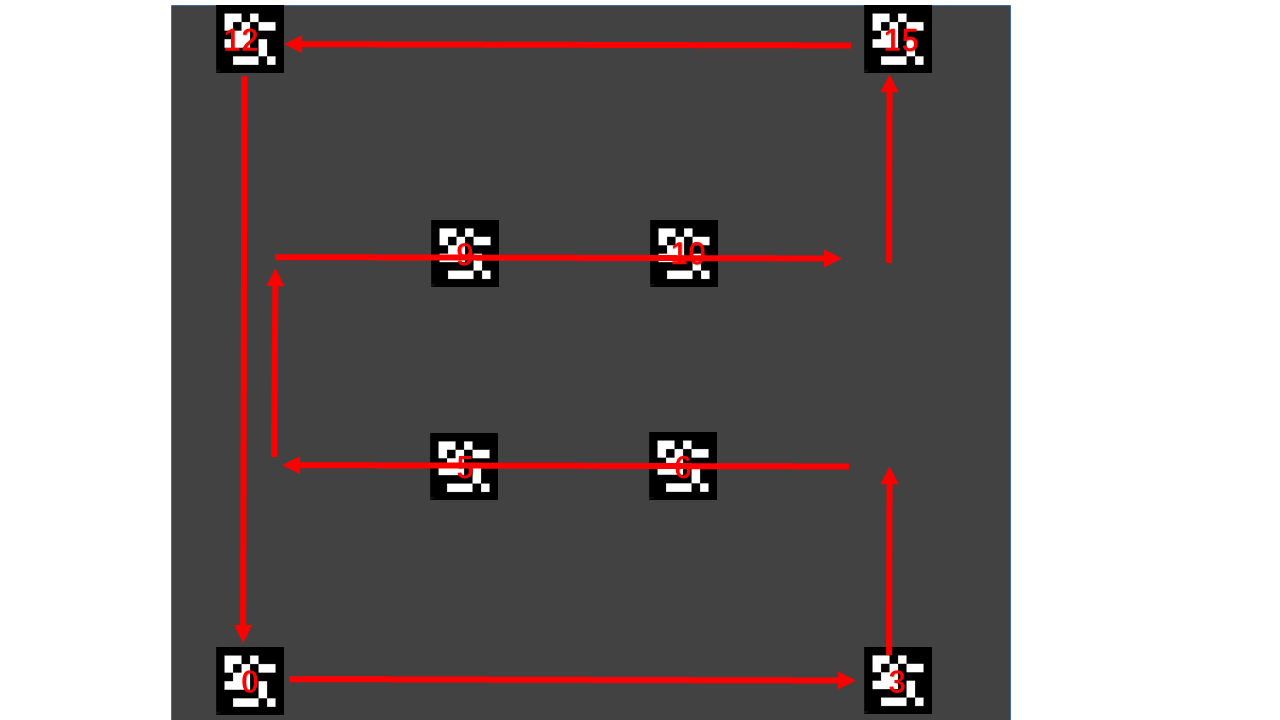
\includegraphics[height=8cm]{flight_route.png}
  \caption{无人机自主飞行轨迹设计图}
  \label{fig:flight_route}
\end{figure}
\subsection{视觉定位系统实验结果分析}
\label{sec:5.2.2}

按照上述实验流程让无人机进行自主飞行,可以直接获取到视觉算法生成的地图以及无人机在飞行的过程中生成的三维坐标,根据这些数据可以对
视觉算法关于无人机自主定位的效果进行定量的分析,本节主要从生成地图的精度,无人机三维坐标的精度以及轨迹精度三个方面进行定量分析。

首先对于地图精度,根据图~\ref{fig:scene_reality}生成的地图,通过对地图的解析,可以获取每一个二维码的三维位置坐标,如
表~\ref{tab:chap1:marker_pose}所示。

\begin{table}[h]
  \centering
  \caption{二维码标志位置实际测量值}
  \label{tab:chap1:marker_pose}
  \begin{tabular}{C{3.6cm}L{2.4cm}L{2.4cm}L{2.4cm}}
  \toprule
  \textbf{序号} & \textbf{X} & \textbf{Y} & \textbf{Z} \\
  \midrule
  0      & -2.63   & 	1.32 & 7 .86            \\
  3      & -14.69  & 	3.88 & 7.80            \\
  5      & -6.05 	 &  6.34 & 7.45           \\
  6      & -9.83 	 &  -9.83 & 7.45           \\
  9      & -5.13 	 &  10.44 & 7.30           \\
  10     & -9.17   &	11.22 &	7.24        \\
  12     & -0.33 	 &  13.56 & 7.34 	             \\
  15     & -12.25  & 	16.15 &	7.27            \\
  \bottomrule
  \end{tabular}
  \end{table}

  针对地图的精度,可以提出以下两个判断指标。\\
  1)任意两个二维码之间距离的测量值和理论值的误差比较;\\
  2)所有二维码是否在同一个坐标平面。
  
针对指标1,计算得到表~\ref{tab:chap1:marker_map_error},经过计算得到地图中二维码的误差精度为3.1$\%$。

  \begin{table}[h]
    \centering
    \caption{二维码位置误差}
    \label{tab:chap1:marker_map_error}
    \begin{tabular}{C{1.6cm}C{1.6cm}C{2.4cm}C{2.4cm}C{3.2cm}}
    \toprule
    \textbf{ID1} & \textbf{ID2} & \textbf{实际值} & \textbf{理论值} & \textbf{误差率} \\
    \midrule
    0&	3&	12.33&	12&	2.75 $\%$\\
    0&	5&	6.07&	5.65&	7.43$\%$\\
    0&	6&	9.26&	8.94&	3.58$\%$\\
    0&	9&	9.46&	8.94&	5.82$\%$\\
    0&	10&	11.86&11.31&	4.86$\%$\\
    0&	12&	12.45&	12&	3.75$\%$\\
    0&  15&	17.67&	16.97&	4.12$\%$\\
    3&	5&	8.99&	8.94&	0.56$\%$\\
    3&	6&	5.85&	5.65&	3.54$\%$\\
    3&	9&	11.6&	11.31&	2.56$\%$\\
    3&	10&	9.18&	8.94&	2.68$\%$\\
    3&	12&	17.32&	16.97&	2.06$\%$\\
    3&	15&	12.51&	12&	4.25$\%$\\
    5&	6&	3.87&	4&	3.25$\%$\\
    5&	9&	4.21&	4&	5.25$\%$\\
    5&	10&	5.79&	5.65&	2.48$\%$\\
    5&	12&	9.21&	8.94&	3.02$\%$\\
    5&	15&	11.61&	11.31&	2.65$\%$\\
    6&	9&	5.75&	5.65&	1.77$\%$\\
    6&	10&	4.13&	4&	3.25$\%$\\
    6&	12&	11.47&	11.31&	1.41$\%$\\
    6&	15&	9.33&	8.94&	4.36$\%$\\
    9&	10&	4.11&	4&	2.75$\%$\\
    9&	12&	5.72&	5.65&	1.24$\%$\\
    9&	15&	9.12&	8.94&	2.01$\%$\\
    10&	12&	9.15&	8.94&	2.35$\%$\\
    10&	15&	5.81&	5.65&	2.83$\%$\\
    12&	15&	12.2&	12&	1.67$\%$\\  
    \bottomrule
    \end{tabular}
    \end{table}

针对指标2,绘制出每个二维码的在同一个坐标平面的误差情况,如图~\ref{fig:marker_map_error_Z}所示,,平均误差为0.18m
可以认定所有二维码基本都在同一水平面内。
    \begin{figure}[H] % use float package if you want it here
      \centering
      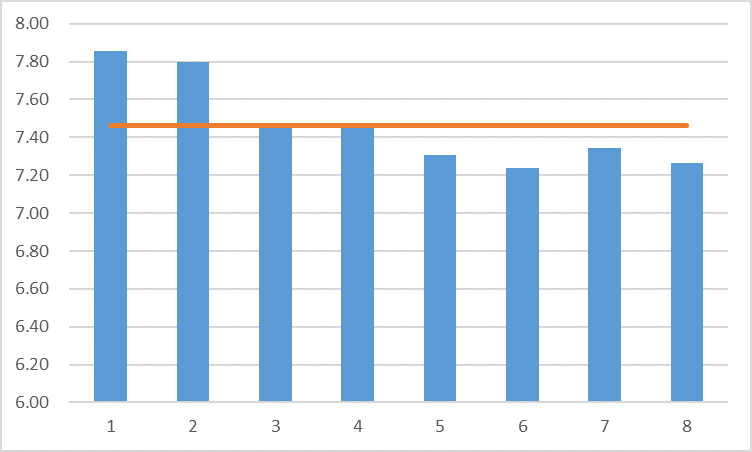
\includegraphics[height=8cm]{marker_map_error_Z.png}
      \caption{二维码Z方向数据}
      \label{fig:marker_map_error_Z}
    \end{figure}
其次对于无人机三维坐标的精度,以无人机自带GPS测距仪器测定出的坐标为真值,和视觉算法计算出来的位置信息进行对比,选择无人机
在0-800帧的数据,在X、Y、Z方向得到的结果分别如图~\ref{fig:chap2:pose_xyz}所示,其中蓝色连线为视觉算法检测出的坐标值,红色
连线无人机GPS检测出的真实值。
\begin{figure}[htbp]
  \centering
    \subcaptionbox{X方向GPS和视觉算法对比图}{\label{fig:chap1:pose_x}
    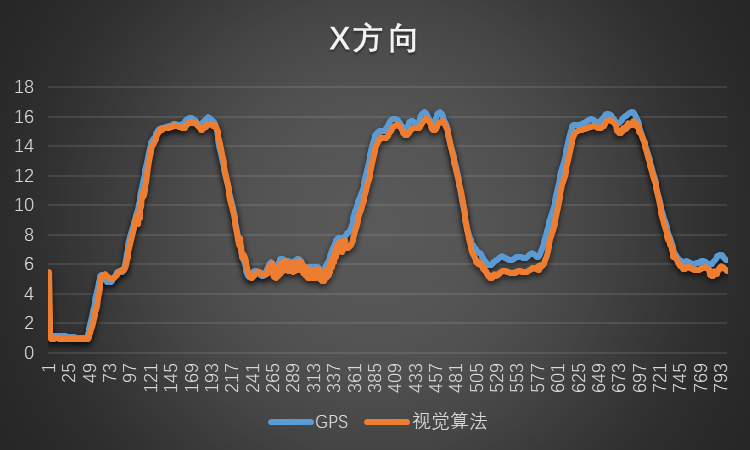
\includegraphics[width=6cm]{pose_x.png}\hskip2cm}
    \subcaptionbox{Y方向GPS和视觉算法对比图}{\label{fig:chap1:pose_y}
    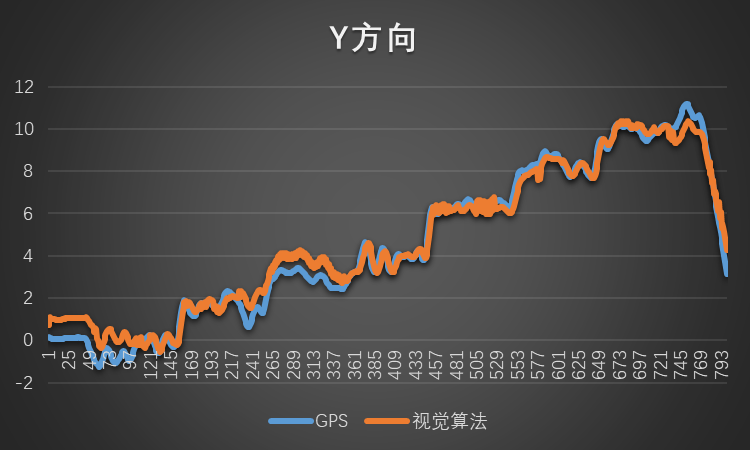
\includegraphics[width=6cm]{pose_y.png}}
  \vskip0.5cm
    \subcaptionbox{Z方向GPS和视觉算法对比图}{\label{fig:chap1:pose_z}
    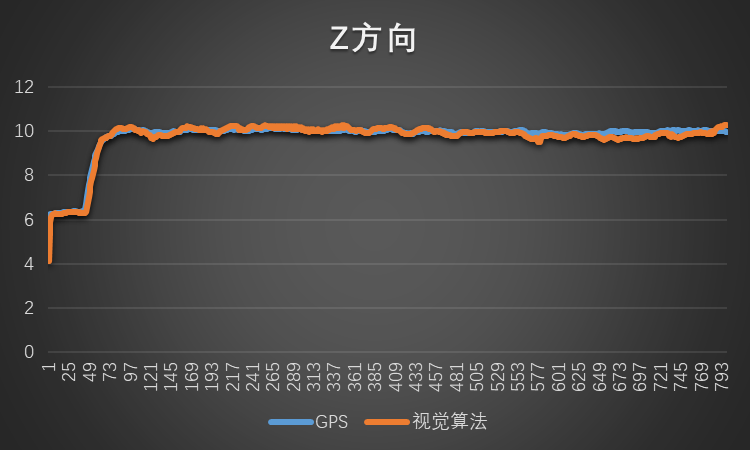
\includegraphics[width=6cm]{pose_z.png}\hskip2cm}
  \caption{各方向GPS和视觉算法对比图}\label{fig:chap2:pose_xyz}
  \end{figure}
随后,计算真值和测量值之间的误差,在X、Y、Z方向分别得到结果如图~\ref{fig:chap2:pose_error_xyz}所示,对于X、Y、Z三个方向分别可以
得到距离误差为0.22m、0.37m、0.107m。
  \begin{figure}[H]
    \centering
      \subcaptionbox{X方向GPS和视觉算法对比图}{\label{fig:chap1:pose_error_x}
      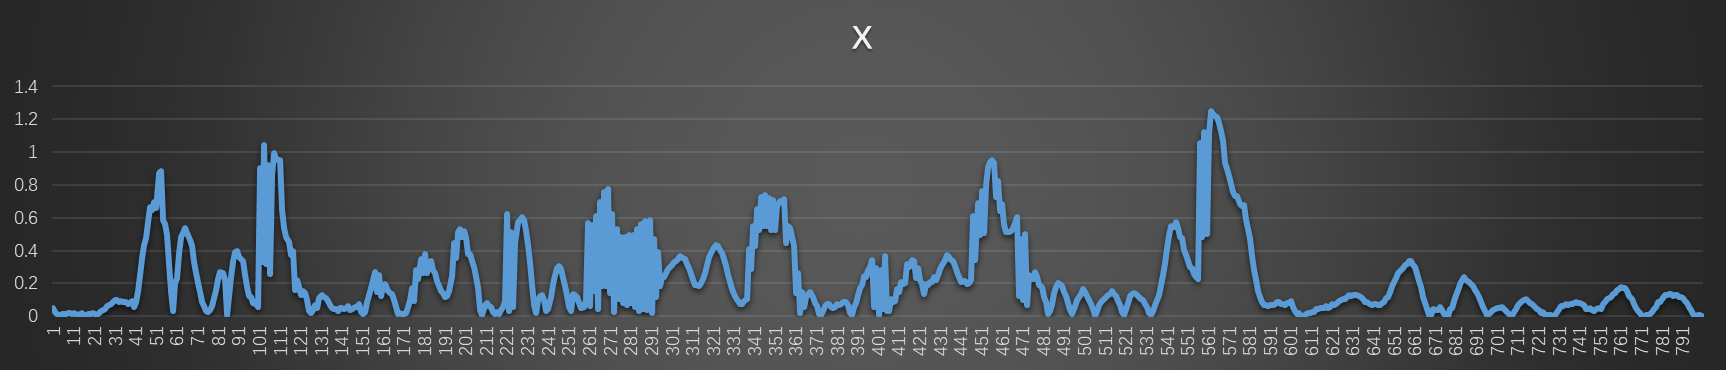
\includegraphics[width=12cm]{pose_error_x.png}}
    \vskip0.5cm
      \subcaptionbox{Z方向GPS和视觉算法对比图}{\label{fig:chap1:pose_error_y}
      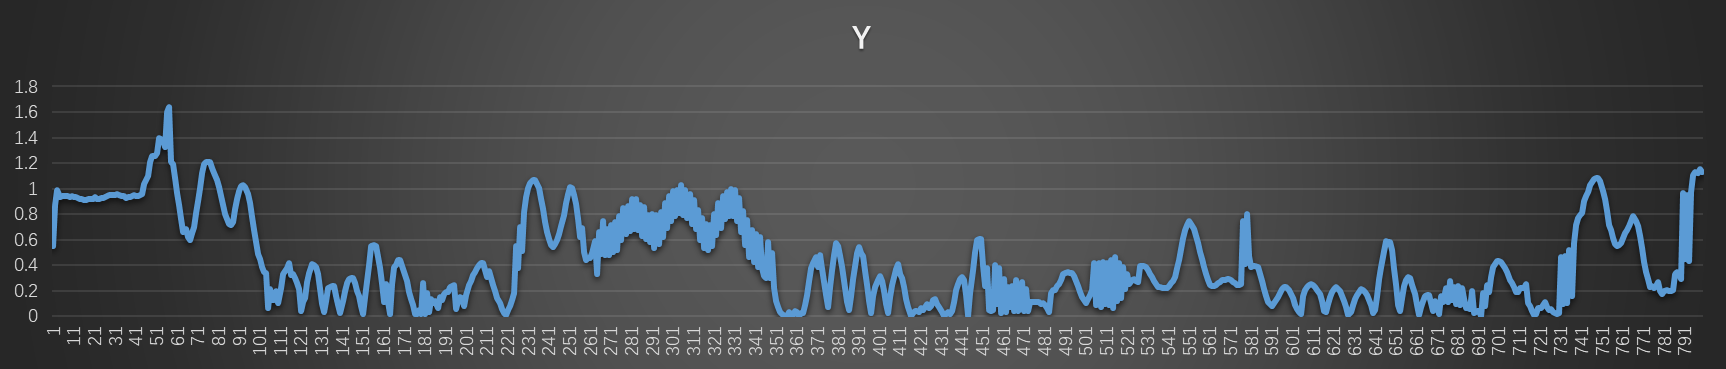
\includegraphics[width=12cm]{pose_error_y.png}}
    \vskip0.5cm
      \subcaptionbox{Z方向GPS和视觉算法对比图}{\label{fig:chap1:pose_error_z}
      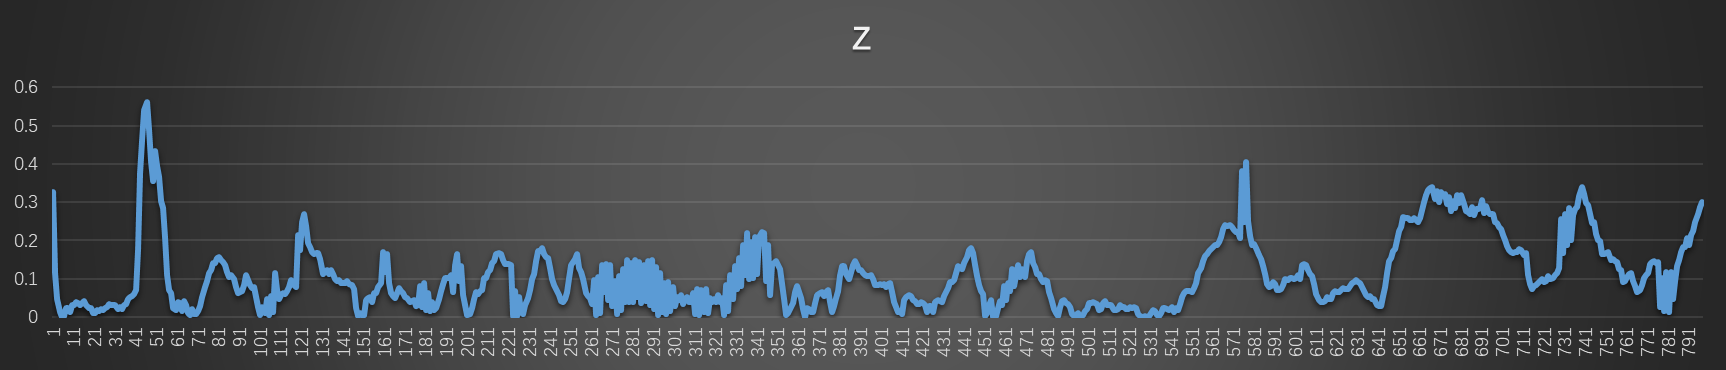
\includegraphics[width=12cm]{pose_error_z.png}}
    \caption{各方向GPS和视觉算法误差对比图}\label{fig:chap2:pose_error_xyz}
    \end{figure}
最后,对无人机的轨迹精度进行对比。无人机在自主飞行过程中能够产生实时的相对于真实世界坐标系的定位信息,将其与GPS生成的定位信息
进行对比,如图~\ref{fig:pose_map}所示。
    \begin{figure}[H] % use float package if you want it here
      \centering
      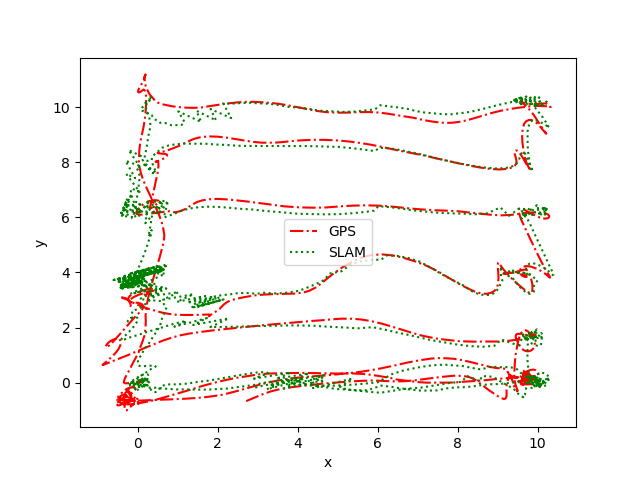
\includegraphics[height=12cm]{pose_map.png}
      \caption{无人机轨迹对比示意图}
      \label{fig:pose_map}
    \end{figure}
    对于无人机的直飞路线,误差较小,GPS和视觉算法测算出的轨迹基本吻合,但是在对于转弯改变方向的区间,两者之间的相对误差则较大,
    考虑其原因为,在转弯处所设计的循迹点相对比较稠密,导致在该区域内无人机需要改变的方向更大,导致视觉算法在测算时由于方法振动、
    的缘故产生较大的误差。